\chapter{绪\hspace{6pt}论}

\section{研究工作的背景与意义}
\subsection{研究背景}

随着信息技术产业的高速发展,数字信息量呈爆炸式增长。国际数据资讯公司(IDC)\cite{IDC}于2020年公布的统计及预测报告\cite{DataReport2020}显示,每年新产生的数据量在2015年至2025年间以约26\%的复合年增长率增长,预计仅2025年创建的新数据数据量将高达175.8\,ZB(而2015年仅为18.2\,ZB)。新创建数据量的快速增长导致个人及企业面临的数据存储和管理成本快速上涨\cite{敖莉2010重复数据删除技术}。另一方面,在各类型存储系统所保存的数据中,高达60\%的数据都是冗余的。并且,随着时间的推移,这些冗余数据占总数据量的比例将进一步上升\cite{mcknight2006digital}。近年来,存储系统中数据高度冗余的特点得到越来越多研究人员的关注,利用该特点来节省存储空间、降低存储管理开销是成为热门研究课题。

重复数据删除(data deduplication)\cite{2012重复数据删除关键技术研究进展, 敖莉2010重复数据删除技术,xia16,Paulo2014} 是一种粗粒度数据压缩技术。传统数据压缩针对小规模数据(例如同一文件内部),使用字节级重新编码以降低冗余;而重复数据删除作用的基本单位是数据块(通常为8KiB),通过比较来自相同和不同文件的数据块,为具有相同内容的数据块仅保存一份物理拷贝以节约存储空间。如图~\ref{fig:Deduplication-storage-pattern}所示,在支持重复数据删除的各类存储系统(统称为重复数据删除系统)中,重复数据删除后的任何数据块都被一个或多个文件引用,而每个文件则以指向这些数据块的指针的集合形式进行存储。重复数据删除可为主存和备份数据分别节省50\%\cite{meyer11}和98\%\cite{wallace12}的存储空间,可显著降低云存储厂商的存储及维护成本\cite{2012重复数据删除关键技术研究进展}。由于能够有效地降低存储开销,重复数据删除技术非常适合为管理日益增长的海量数据节省成本。在工业界,Dell EMC Data Domain\cite{EMCDataDomain}、Avamar\cite{Avamar}、Veritas的NetBackup Appliances\cite{veritas} 以及Commvault的开放数据平台\cite{CommVault} 都是较为知名的重复数据删除应用产品;此外,各大云存储厂商(例如 Dropbox\cite{Dropbox}、Google Drive\cite{GoogleDrive}、百度网盘\cite{BaiduPan}等)也纷纷将重复数据删除技术应用于各自的云服务产品中,以提升经济效益\cite{harnik2010side}。  

\begin{figure}[!htb]
    \small
    \centering
    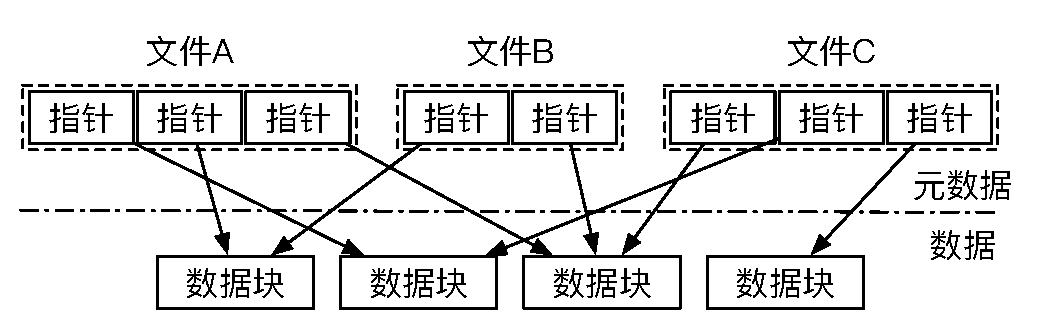
\includegraphics[width=0.75\textwidth]{pic/DedupSystemStorageMode.eps}
    \caption{重复数据删除系统的存储模式} 
    \label{fig:Deduplication-storage-pattern}
\end{figure} 

\textbf{本文重点关注面向云环境的重复数据删除}。图~\ref{fig:Cloud-based-deduplication-storage-logic}描述了云环境重复数据删除系统框架。云服务商维护哈希索引表,记录所有已存储数据块的哈希值。在重复数据删除过程中,用户使用云存储客户端计算目标数据块的哈希值;云服务商检查该哈希值是否存在于数据块索引表中,如果哈希值存在(即云端已有目标数据块的副本),则更新目标数据块的所有权信息并通知客户端无需传输该数据块,从而同时节省传输带宽和存储空间(这种重复数据删除方式称为源端重复数据删除(source-based deduplication))。然而,由于重复数据删除系统中任意重复数据块均只保留一个副本,任意一个数据块的泄露可能扩散影响到共用该数据块的所有文件。这种文件共用数据块的存储模式强调了数据块的敏感性。因此,如何保护重复数据删除后的数据的隐私,成为云存储服务商应用重复数据删除技术亟需解决的关键问题。

\begin{figure}[!htb]
    \small
    \centering
    \includegraphics[width=\textwidth]{pic/Cloud-deduplication.pdf}
    \caption{云环境重复数据删除系统结构} 
    \label{fig:Cloud-based-deduplication-storage-logic}
\end{figure} 

近年来,研究者提出加密后重复数据删除\cite{bellare2013MLE}以保护重复数据删除过程中的数据安全。图~\ref{fig:Cloud-based-encrypted-deduplication-storage-logic}描述了加密后重复数据删除系统框架,其包括客户端和云服务端两个主要组成部分。为了防止云服务商获取外包数据内容,加密后重复数据删除系统在客户端部署消息锁加密(MLE:message-locked encryption)\cite{bellare2013MLE}以加密明文数据块(简称为明文数据块),同时确保重复数据删除仍然能够作用于密文数据块(简称为密文数据块)以节约存储空间。传统对称加密算法为每个客户端或每个数据块分配不同加密密钥,导致相同的明文数据块被加密为不同的密文数据块,无法通过重复数据删除进行冗余消除。消息锁加密的核心思路时基于数据块内容产生密钥(称为MLE密钥,例如MLE密钥为明文数据块的哈希值\cite{douceur02}),从而将相同明文数据块加密为相同的密文数据块,以兼容直接针对密文数据块的重复数据删除。现有消息锁加密采用服务器辅助密钥生成方式(称为服务器辅助消息锁加密(Server-aided MLE)
\cite{keelveedhi2013DupLESS}),即部署第三方密钥服务器管理全局秘密,同时基于明文数据块哈希值以及密钥服务器的全局秘密共同生成MLE密钥,以防止攻击者针对MLE密钥实施离线暴力破解攻击。

\begin{figure}[!htb]
    \small
    \centering
    \includegraphics[width=\textwidth]{pic/Cloud-encrypted-deduplication-logic.pdf}
    \caption{面向云环境的加密后重复数据删除系统框架}
    \label{fig:Cloud-based-encrypted-deduplication-storage-logic}
\end{figure}

另一方面,重复数据删除受到伪造数据所有权的攻击威胁\cite{harnik10,mulazzani11}。由于云服务商仅基于收到的数据块哈希值判断客户端是否拥有相应数据块,恶意用户/客户端可以伪造任意密文数据块的哈希值,如果该密文数据块已在云端存储(即已发生重复数据删除),则恶意客户端无需传输密文数据块内容便可获得相应密文数据块的访问权限。为了防止伪造所有权攻击,加密后重复数据删除增加了所有权证明(proof-of-ownership)技术\cite{halevi11}:除了密文数据块的哈希值以外,云服务商要求客户端额外提交目标密文数据块的所有权证明(proof);云服务商首先基于证明验证该客户端是否真实且完整拥有相应密文数据块,然后再执行如前所述的重复数据删除过程。所有权证明技术的合理性在于,只针对客户端真实拥有(即具有完整访问权限)的密文数据块执行重复数据删除,从而避免非法访问其他客户端的已存储内容。

然而,支持数据块所有权证明技术的加密后重复数据删除依然不足以完全击败恶意客户端,恶意客户端仍可通过枚举数据块内容以发起推测内容攻击({\em learning-content attack})\cite{harnik10, zuo18}。具体来说,攻击者对目标文件具有相当的先验知识,了解目标文件(例如,来自同一家公司的录用通知书)的大部分格式化内容,并旨在识别其他客户拥有的目标文件的私有部分(例如,录用通知书中的签约工资和入职奖金数额)。攻击者通过枚举目标文件中私有内容的可能值来伪造大量文件,对每个伪造的文件执行源端重复数据删除,进而在某些伪造的文件无需上传任何内容时推断出目标文件中的隐私信息(即当前伪造文件所包含的内容)。

\subsection{问题和动机}

现有面向云环境的加密后重复数据删除系统面临着系统效率低与安全性不足的双重挑战:

\paragraph{系统效率} 

在服务器辅助密钥生成过程中,现有加密后重复数据删除系统(图~\ref{fig:Cloud-based-encrypted-deduplication-storage-logic})须使用基于盲签名[8][2]的无记忆伪随机函数(OPRF:oblivious pseudorandom function)生成密钥[8],以防止密钥服务器获得明文块的哈希值。同时,为了实现所有权证明,系统须在云服务端维护Merkle哈希树,并基于哈希树验证客户端提交的证明信息[19]。项目组指出,服务器辅助密钥生成和所有权证明的密码操作是加密后重复数据删除系统的主要效率瓶颈。
为了验证以上论断,项目组基于图1框架和现有技术方案实现了加密后重复数据删除系统的基础原型。基础原型支持基于RSA[8]或BLS[2]盲签名生成密钥,以及基于Merkle哈希树[19]或通用哈希(universal hash)[45]证明所有权(注:基于通用哈希的所有权证明方法[45]只能达到较低安全性)。

表1展示了基础原型每个步骤处理1MiB数据的平均时间开销。服务器辅助密钥生成是最大效率瓶颈。如果采用基于Merkle哈希树的所有权证明方案,RSA盲签名和BLS盲签名分别占系统总开销的53.8\%和93.3\%。同时,所有权证明也是限制系统效率的重要因素,如果采用基于RSA盲签名的服务器辅助密钥生成方案,Merkle哈希树和(较低安全性的)通用哈希方案分别占系统总开销的35.7\%和9.5\%。

\paragraph{安全隐患} 

在重复数据删除过程中,云服务商通知客户端传输或不传输密文块内容(§1.1),实质上泄漏了“其他客户端是否已经存储相应密文块”的侧信道信息(side-channel information)。虽然所有权证明阻止了针对非授权密文块的重复数据删除,但不足以防止恶意客户端的侧信道攻击。
例如,攻击者可以枚举所有可能的数据内容,并利用重复数据删除泄漏的侧信道信息实施推测内容攻击(learning-content attack)[20][50]。假设攻击者已知某个客户端持有目标文件且文件内容符合固定的公开格式(例如工资条、合同等模版化数据),致力于推断目标文件未公开的敏感内容(例如薪水金额)。攻击者枚举所有可能的未公开内容,并通过恶意客户端上传所生成的枚举文件。如果上传某个枚举文件时无需传输任何密文块,即可推断该枚举文件即为目标文件。此时,由于攻击者完全获得了所枚举文件的访问权限,仅检测所有权无法阻止推测内容攻击。
项目组扩展现有工作[20][50],设计案例验证推测内容攻击的可行性。考虑Alice和Bob为应届毕业学生,同时收到某公司的雇佣合同。他们将各自合同备份至云端。假设Alice为攻击者,通过推测内容攻击推断Bob合同中的薪水和签字费。
为了实现以上案例,项目组基于Google合同模版[58],更改其中姓名、年薪(假设为6K的倍数[20],介于204K和804K之间)和签字费(假设为10K的倍数,介于300K和600K之间)以生成Alice和Bob的合同,每个合同约占18.5KiB。项目组随机生成Bob的薪水和签字费,并通过基于图1设计实现的基础原型将Bob的合同存储至服务端。令Alice基于自身合同作为内容模版,枚举Bob所有可能的薪水和签字费,以实施推测内容攻击。项目组分别在本地局域网(客户端、密钥服务器和服务端均部署在具有10Gb/s网速的本地实验环境)和阿里云(在本地部署客户端和密钥服务器,在阿里云部署服务端)实现上述攻击。Alice需上传大约841份伪造合同,消耗7.4MiB网络流量(包括传输非重复密文块和元数据),在局域网和阿里云环境中推断Bob的隐私信息分别只需105.0秒和475.5秒。
  

\subsection{研究意义}

\section{国内外研究历史与现状}

\subsection{加密后重复数据删除}
\subsubsection{加密后重复数据删除技术}
\subsubsection{服务器辅助密钥生成}
\subsubsection{所有权证明技术}
\subsection{可信计算平台}
\subsubsection{Intel SGX}
\subsubsection{AMD SEV}
\subsubsection{ARM Trusted Zone}


\section{本文的主要贡献与创新}

\section{本论文的结构安排}